\documentclass[12pt]{article}
\usepackage{xcolor} % for different colour comments


%\usepackage{refcheck}
\newif\ifcomments\commentstrue

\ifcomments
\newcommand{\authornote}[3]{\textcolor{#1}{[#3 ---#2]}}
\newcommand{\todo}[1]{\textcolor{red}{[TODO: #1]}}
\else
\newcommand{\authornote}[3]{}
\newcommand{\todo}[1]{}
\fi

\newcommand{\wss}[1]{\authornote{magenta}{SS}{#1}}
\newcommand{\ds}[1]{\authornote{blue}{DS}{#1}}


\usepackage{hyperref}
\usepackage{graphicx}
\usepackage{verbatim} 
\graphicspath{ {Images/} }


\begin{document}

\title{Smart Waiter Test Plan} 
\author{Meraj Patel \#1137491 \\ Pavneet Jauhal \#1149311\\ Shan Perera \#1150394}
\date{\today}
\maketitle

\pagebreak

\tableofcontents

\listoftables
\section*{Revision History}
\begin{tabular}{|p{5cm}|p{5cm}|}
\hline
\textbf{Date}  & \textbf{Comments} \\ \hline
October 30, 2015 &  first draft. \\ 
February 1, 2016 &  Added usability questions \\ 
April 15, 2016 &  Addressed Dan's comments in regards to spelling and grammar. Modified automated testing \\ 
April 16, 2016 &  Addressed more Dan's comments in regards to spelling and grammar. Fixed tables. Added item selection and customization\\ 
\hline
\end{tabular}

\pagebreak

\section{Document Changes}
\begin{itemize}
 \item Updated testing tables according to Dan's comments. As well, added more test cases. This is seen in: 
 \begin{itemize}
 \item Section 6: Database testing
 \item Section 7.1: Barcode Scanning (now includes deprecated barcodes)
 \item Section 7.2: Account Sign up and Login
 \item Section 7.3: Item Selection and Customization (new)
 \end{itemize}
 \item Added table figure numbers.
 \item Added testing schedule (section 8)
 \end{itemize}

%%%%%%%%%%%%%%%%%%%%%%%%
%
%	1.) General Information 
%
%%%%%%%%%%%%%%%%%%%%%%%%

\section{General Information}
The following section provides an overview of the test plan 
for Smart-Waiter.This section explains the purpose of this document, the scope of the system, and an overview of the following sections.

%1.1 Purpose
\subsection{Purpose}
The purpose of this document is to describe  various test cases and procedures to evaluate functionality of Smart Waiter.
This document is indented to be used as a reference for all future testing. 

%1.2 Scope
\subsection{Scope}
This test plan is used to evaluate Smart Waiter functionality. Various plans are described in detail to test expected functional and non function requirements.  

\subsection{Overview of Document }
The following sections provide more detail about types of test that will be used. Information about the testing process is provided, and the software specifications
that were discussed in the requirements document are stated. Testing processes are split up between system test for POC and the final demonstration. 

\subsection{Acronyms}
\begin{description}
\item[SRS] Software Requirements Specification
\item[POC] Proof of concept demonstration
\end{description}

%%%%%%%%%%%%%%%%%%%%%%%%
%
%	2.) Plan
%
%%%%%%%%%%%%%%%%%%%%%%%%

\section{Plan}
This section provides a description of the software that is being tested, the team that will
perform the testing, and milestones for the testing phase.

%2.1 Software Description
\subsection{Software Description}
Smart-Waiter aims to provide a solution that will allow users to order and pay through a mobile application at restaurants. 

%2.2 Test Team
\subsection{Test Team} 
Team members who will write, review and execute test cases for Smart Waiter are: 

\begin{itemize}
 \item Pavneet Jauhal
 \item Shan Perera
 \item Meraj Patel
 \item Dr.\ Rong Zheng
\end{itemize}  

%2.3 Milestones
\subsection{Milestones}

%2.3.1 Location
\subsubsection{Location}
The location where testing will be performed is McMaster University, Hamilton Ontario.


%2.3.1 Dates and Deadlines
\subsubsection{Dates and Deadlines}

Test Case Creation:
Creation of POC test cases begin October 19, 2015, and is expected to end November 16, 2015. Proceeding, test cases for final demonstration will be created and finished by February 1, 2016.
\newline
\newline
Test Case Implementation:
Implementing test cases for POC system test is scheduled to begin November 15, 2015 and will be completed in approximately one week.
\newline
\newline
Implementing test cases for Final Demonstration system test is scheduled to begin February 1, 2016, and will be completed in approximately three weeks. 


%%%%%%%%%%%%%%%%%%%%%%%%
%
%	3.) Software Specification
%
%%%%%%%%%%%%%%%%%%%%%%%%

\section{ Software Specification}
This section provides; the functional requirements the 
software is expected to complete, and the non-functional requirements the software is expected to exhibit.

%3.1 Functional Requirements
\subsection{Functional Requirements}

\noindent
\begin{itemize}
\item The product shall scan a bar code to access the restaurant menu from a database
\item The product shall allow the user to register an account for complete access to payment services
\item The product will allow users to add and customize items to cart
\item The product will allow users to place their order
\item The product will allow users to pay for their order using a credit card
\end{itemize}  

%3.2 Nonfunctional Requirements
\subsection{Nonfunctional Requirements}
Priority non functional requirements are:
\begin{itemize}
\item Performance
\item Ease of use
\item Reliability
\item Security
\item Maintainability
\end{itemize} 
%%%%%%%%%%%%%%%%%%%%%%%%
%
%	4.) Test Types
%
%%%%%%%%%%%%%%%%%%%%%%%%

\section{Evaluation}

The following section presents methods and constraints used during the evaluation process, and is followed by extent of testing and test tools to be used.

%4.1 Methods and Constraints
\subsection{ Methods and Constraints} 

%4.1.1 Methodology
\subsubsection{Methodology} 
Testing of Smart Waiter will consist of various types of tests explained in the next section. Manual testing will be conducted for the most part, some automation testing will be in place.

% 4.1.2 Extent of Testing
\subsubsection{Extent of Testing}
The extent of testing will be end to end for the final demonstration. As for POC, specific system tests will be conducted.

% 4.1.3 Test Tools
\subsubsection{Test Tools}
To avoid regressions and catch bugs the following tool will be used:
\begin{itemize}
\item CodeReviewer \textemdash CodeReviewer will be used for code review process mandatory for all developers. This tool helps post code reviews and provides features such as annotations, diff viewers, easy communication and feedback. This tool will be used for static tests to produce high quality code with less defects
 \end{itemize}

% 4.1.4 Testing Constraints
\subsubsection{ Testing Constraints}
N/A

\subsection{Types of Tests}

\subsubsection{Functional Testing}
Functional testing is in place to uncover errors that occur in implementing requirements or design specifications. Concentration is on results rather than internals functions of the program. This type of testing is very useful to evaluate functional requirements.

\subsubsection{Structural Testing}
Structural testing is in place to uncover errors during the implementation of the application. Concentration is on evaluating the structure of the application. This type of testing focuses on nonfunctional requirements.   

\subsubsection{Unit Testing}
Unit testing refers to providing specific input to a system and verifying it evaluates to expected output. This process can be done manually or can be automated.

\subsubsection{Manual and Automatic Testing}
Manual testing is done by people, while automatic is processed through scripts. 

\subsubsection{Static Testing}
Static testing refers to testing techniques that simulate a dynamic environment. This does not involve program execution. Instead, a walk-through will be performed checking pre and post conditions evaluate to requirements specified. As well to make sure the proper syntax is used thoroughly. This type of testing is crucial in the design stage. \\
Static testing will be enforced throughout the development process. A code review process will be put in place to manage the quality of the code. Specifically, developers will have to sign off on the quality of the code before it gets checked into the production repo.
\begin{figure}[!htb]
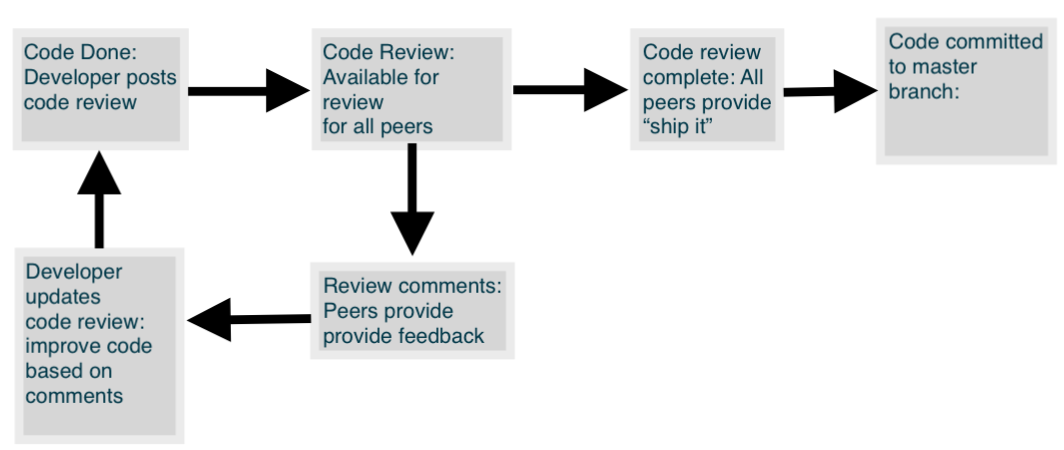
\includegraphics[width=\textwidth,height=\textheight,keepaspectratio]{review_process.png}
\caption{Code Review Process}
\label{fig:CodeReview}
\end{figure}
\\\\
The reviewers will assess the code quality and critique the code in following criteria:\\
\begin{itemize}
 \item General Unit Testing performed. Did it pass?
 \item Comment and Coding Conventions followed consistently?
 \item Error Handling done correctly?
 \item Resource Leaks within the code?
 \item Is the code thread safe?
 \item Is the code up to standard with performance?
 \item Does code provide correct functionality?
 \item Is the code secure?
 \end{itemize}
Reviewers will assess the code and mark issues found with severity. If high severity issues exist, then the developer must fix the system immediately. Medium and low severity issues can be addressed at a later time. The reviewers will mark severity as follows;
\begin{itemize}
\item Naming Conventions and Coding style considered low severity
\item Control flow and logical issues considered medium or high severity
\item Redundant code considered medium or high severity
\item Performance issues considered high severity
\item Security issues considered high severity
\item Scalability issues considered medium or high severity
\item Functional issues considered high severity
\item Error Handling considered high severity
\item Reusability considered medium severity
\end{itemize}

\subsection{Dynamic Testing}
On the contrary, dynamic testing refers to executing the program while running test cases to view expected behavior. This is performed to locate and fix defects in the program. This will be performed after implementation phase. All of the tests completed in the following sections are dynamic. Specifically, different techniques are used to perform this testing such as automated and manual test cases. 

%%%%%%%%%%%%%%%%%%%%%%%%
%
%	5.) System Test Description
%
%%%%%%%%%%%%%%%%%%%%%%%%

\section{POC System Test Description}

%%%%%%%%%%%%%%%%%%%%%%%%%%%%%%%%%%%%%%%%
						%database design %
%%%%%%%%%%%%%%%%%%%%%%%%%%%%%%%%%%%%%%%%
\subsection{Database Testing}
Database testing is exclusively performed from structural testing point of view. The goal of this component of testing is to verify that the database queries always return valid and correct data, under all circumstances. Specifically, a separate database will be created for testing purposes, because any failed test case should not affect the state of the original database. 
\subsubsection{Test Factors}
For database testing, the following test factors will be considered;
\begin{itemize}
 \item Correctness
 \item Performance
 \item Security
 \item Reliability
 \end{itemize}
 
\subsubsection{Correctness}
In this section, the tester must verify that the application receives complete and correct data from the Couchbase server. Automated unit tests will be written using Bash scripts to perform the following tests.
\subsubsection{Database Correctness Automated Tests }
\begin{table}[h]
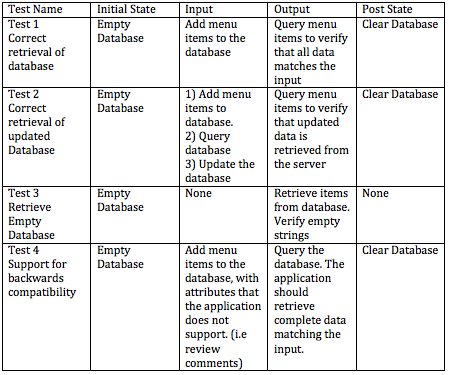
\includegraphics[width=\textwidth,height=\textheight,keepaspectratio]{correctness_tests.png}
  \caption{Database Correctness}
  \label{tbl:excel-table}
\end{table}
\subsubsection{Performance}
In this section, the tester must verify that the data query is performed in a reasonable amount of time. The application should have a maximum loading period of 1.5 seconds to complete data queries. Moreover, considering the customer base and size of database our application, none of the following test cases should take more than 1.5 seconds.

\subsubsection{Database Performance Automated Tests }
\begin{table}[h]
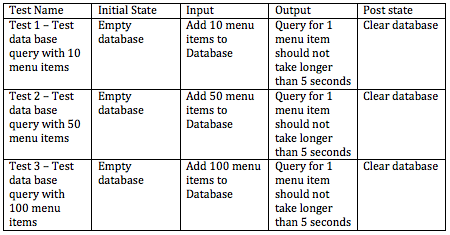
\includegraphics[width=\textwidth,height=\textheight,keepaspectratio]{performance_tests.png}
  \caption{Performance Automated Tests}
\end{table}

\subsubsection{Security}
In this section, the tester must verify that database allows correct access control. Database penetration testing is not required because we will leverage Couchbase security, testing and certifications.
\subsubsection{Database Security Automated Tests }
\break
\begin{table}[h]
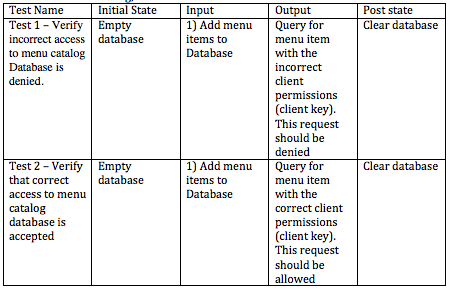
\includegraphics[width=\textwidth,height=\textheight,keepaspectratio]{security_tests.png}
  \caption{Security Test}
\end{table}

\subsubsection{Reliability}
In this section, testing is performed to measure the robustness and reliability of the database.  This type of testing is essential the health of the database system. There should be no failures or downtimes on the back-end side. 
\subsubsection{Database Reliability Automated Tests }
\pagebreak
\begin{table}[h]
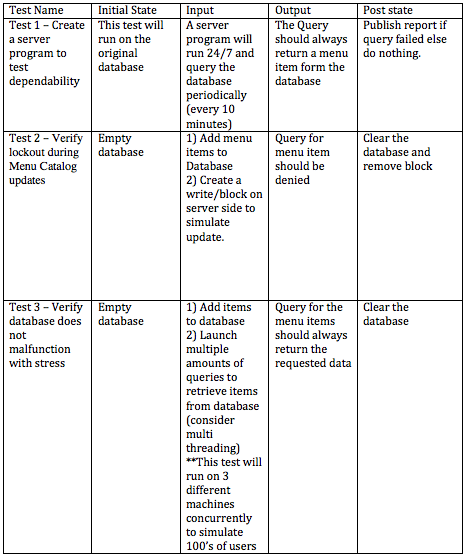
\includegraphics[width=\textwidth,height=\textheight,keepaspectratio]{reliability_tests.png}
  \caption{Reliability Automated Tests}
\end{table}

\section{Final Demonstration System Test Description}

\subsection{Barcode Scanning}
Smart-Waiter needs to ensure users can scan a barcode with minimal attempts. The number of expected attempts will be presented in the final SRS document.

\subsubsection{Test Type}
\begin{itemize}
  \item Manual
  \item Functional test
  \item Unit test
\end{itemize}

\subsubsection{Nonfunctional Test Factors}
\begin{itemize}
  \item Performance
  \item 	Correctness
  \item 	Ease of use
\end{itemize}

\begin{comment}
\subsubsection{Inputs}
\begin{itemize}
  \item Barcode to be scanned
\end{itemize}
\subsubsection{Outputs}
\begin{itemize}
  \item Restaurant menu queried from database
\end{itemize}
\subsubsection{Initial State}
\begin{itemize}
  \item Barcode scanning page in empty state
\end{itemize}
\end{comment}

\subsubsection{Methods of testing}
Dynamic testing is used to ensure correctness and data integrity, and to observe the application behaviour when given incorrect information.

\subsubsection{Test Cases}
\textbf{\textit{Functional Unit Test}}\newline
\newline
\textit{Summary}\newline
Manual black box tests will be performed to assess barcode scanning. This test will be in the form of unit testing. Various test cases described below will be conducted. This is effective as it replicates real world usage and will provide a census of expected number of successful attempts to evaluate nonfunctional test factors.
\newline
\begin{table}[h]
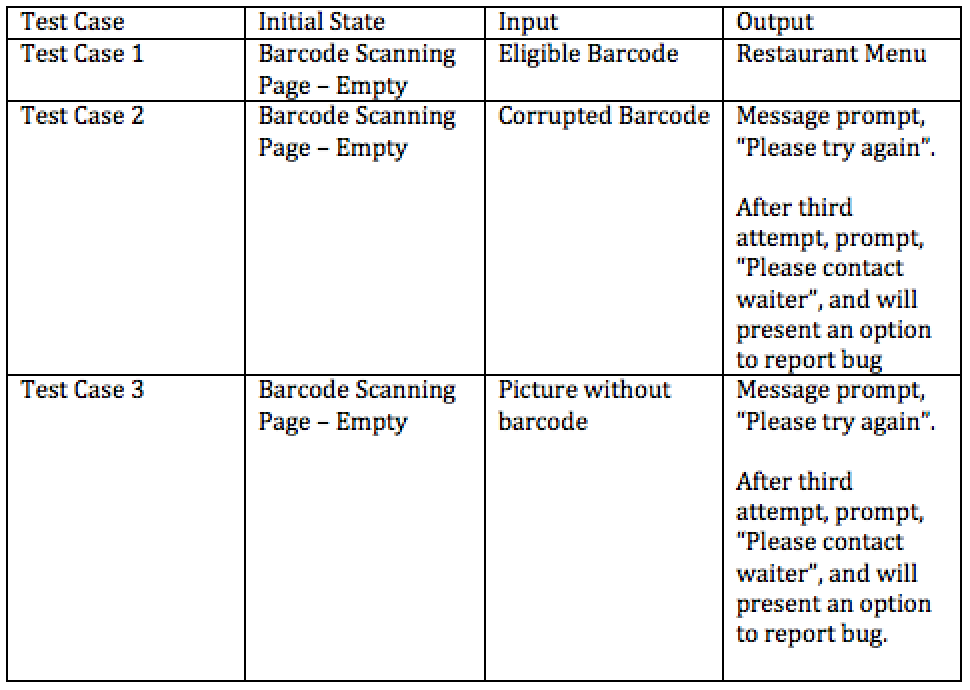
\includegraphics[width=\textwidth,height=\textheight,keepaspectratio]{barcode.png}\newline
  \caption{Barcode Scanning Test}
\end{table}

\subsection{Account Sign up and Login}
Smart-Waiter must use accounts to keep track of a user's personal information. The account module has to provide a secure login service. 
\subsubsection{Test Type}
\begin{itemize}
  \item Manual
  \item functional dynamic test
\end{itemize}
\subsubsection{Nonfunctional Test Factors}
\begin{itemize}
  \item Correctness
  \item data integrity
\end{itemize}


\subsubsection{Methods of testing}
Dynamic testing is used to ensure correctness and data integrity. As well to observe the application behaviour when given incorrect information.
\subsubsection{Test Cases}
\textbf{\textit{Dynamic Testing}}\newline
\newline
\textit{Summary}\newline
Manual dynamic tests will be performed to evaluate the account creation module. This test will be in the form of structural testing. Tests performed on the module are presented below. 
\pagebreak
\begin{table}[h]
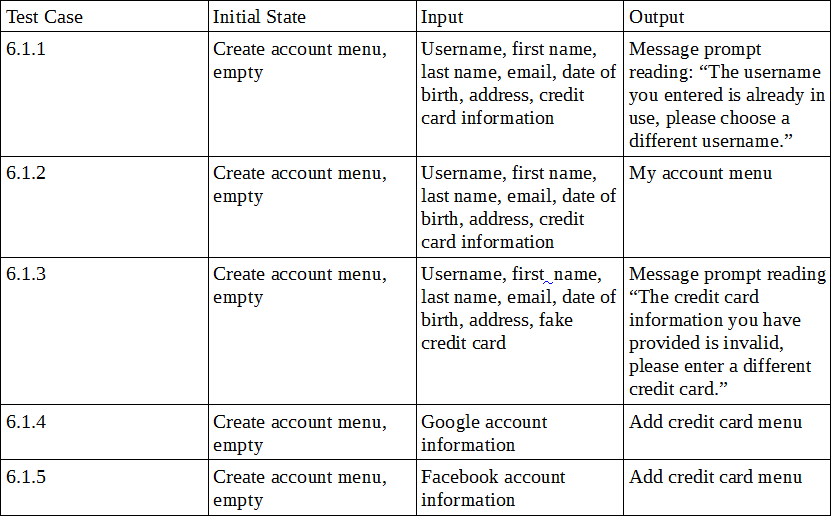
\includegraphics[width=\textwidth,height=\textheight,keepaspectratio]{accountTC.png}
  \caption{Account Sign up and Login Test}
\end{table}
\subsection{Item Selection and Customization}
Smart-Waiter needs to ensure a user is able to select, customize and add item to cart. 

\subsubsection{Test Type}
\begin{itemize}
  \item Manual 
  \item Functional dynamic test 
 \end{itemize} 
 
\subsubsection{Functional Test Factors}
\begin{itemize}
  \item The product shall allow the user to customize and add items to cart
 \end{itemize} 
 
\subsubsection{Methods of testing}
Item selection and customization is performed using  dynamic unit testing. The goal of this component is to verify if a user can select, customize and add multiple menu items to cart. Also, testing is performed to check if a user is able to re-modify an already selected item.  Testing is performed from a functional view to evaluate functional requirements stated in SRS.

\subsubsection{Test Cases}
\textbf{\textit{Dynamic Unit Test}}\newline
\newline
\textit{Summary}\newline
Manual black box tests will be performed to assess item customization and for the ability to add to cart. This test will be in the form of unit testing. Various test cases described below will be conducted. This is effective as it replicates real world usage and will provide a census of expected number of successful attempts to evaluate functional test factors.


\begin{table}[h]
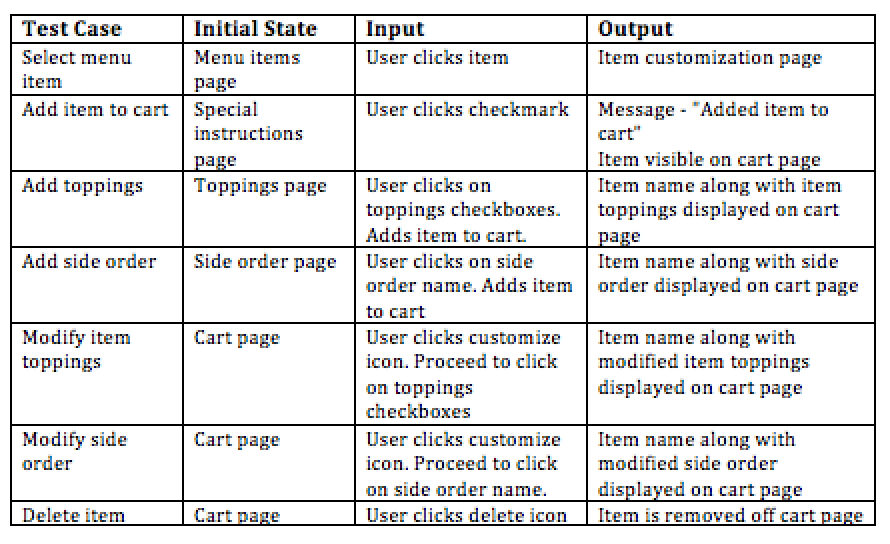
\includegraphics[width=\textwidth,height=\textheight,keepaspectratio]{itemselection.png}
  \caption{Item Selection and Customization Test Cases}
\end{table}

\subsection{Order Transaction}
Smart-Waiter needs to ensure that a user can send in their order, and pay for their order easily and securely. Order transaction will be vigorously tested to ensure complete customer satisfaction.  
\subsubsection{Test Type}
\begin{itemize}
  \item Manual 
  \item functional dynamic test 
 \end{itemize} 
\subsubsection{Nonfunctional Test Factors}
\begin{itemize}
  \item Correctness 
  \item Reliability 
  \item Data integrity 
  \item Data security 
  \item Ease of use
 \end{itemize} 
 

\begin{comment}
\subsubsection{Inputs}
A set \texorpdfstring{n\textsubscript{i}}{ni} of 10 random orders consisting of different menu items, created manually, where i = 0, 1, 2 .. 9, where i = 0..4 are invalid orders with respect to the restaurant's policies and where i = 5..9 are valid orders. \\
A valid credit card \\
An expired credit card \\
A fake credit card \\
A VISA debit card \\
A VISA gift card \\
\subsubsection{Outputs}
An order summary \texorpdfstring{O\textsubscript{i}}{Oi}, where i corresponds to the \texorpdfstring{i\textsuperscript{th}}{ith} order from the set of orders \texorpdfstring{n\textsubscript{i}}{ni}. \\
A message M, containing either a success or failure message, depending on the card type used. 

\subsubsection{Initial State}
Order Test Cases: Restaurant menu module
Credit Card Test Cases: Payment confirmation menu
\end{comment}

\subsubsection{Methods of testing}
Dynamic testing is used to ensure validity, record the number of successful tests given a sample.
\subsubsection{Test Cases}
\textbf{\textit{Dynamic Testing}}\newline
\newline
\textit{Summary}\newline
Manual dynamic tests will be performed to evaluate the order transaction module. This test will be in the form of structural testing. It will test vigorously for all possible inputs of credit card information and account details. The tests being performed on the module are presented below. 
\newline

\begin{table}[h]
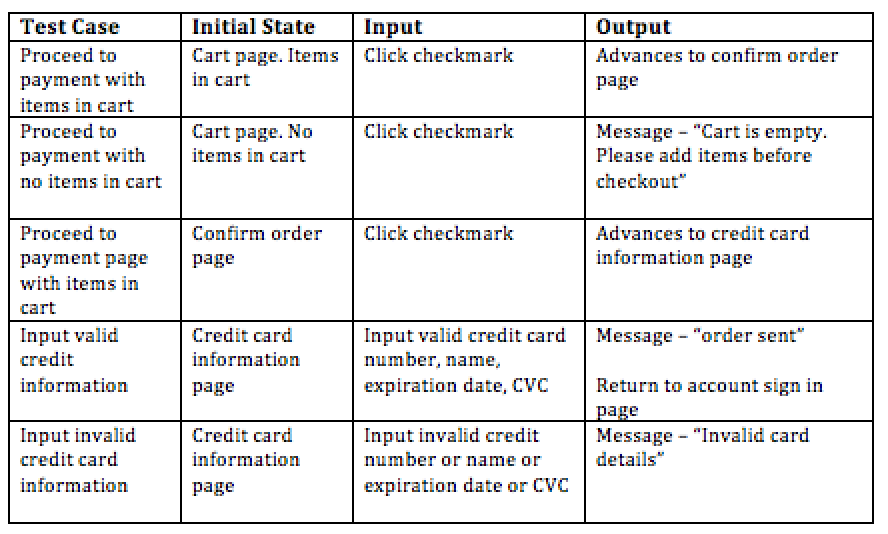
\includegraphics[width=\textwidth,height=\textheight,keepaspectratio]{orderTransactionTC.png}
  \caption{Order Transaction Test Cases}
\end{table}
\subsection{Usability Testing}
The goal of usability testing is to verify if a user can successfully use all functionalities of the application from start to finish in a timely manner. This type of testing aids in evaluating if functional requirements are met. As well it provides scope for evaluating non functional requirements.
\subsubsection{Nonfunctional Test Factors}
\begin{itemize}
  \item Reliability 
  \item Performance
  \item 	Correctness
  \item 	Ease of use
\end{itemize}

\subsubsection{Methods of testing}

Manual black box tests will be performed to assess usability of the application. This test will be in the form of unit testing. 
\\\\
Six participants will be selected to evaluate this test. At least three will have some experience with using android applications. The remaining will have little to no experience. Each participant will be asked to conduct a walk through of the application and complete set tasks. Afterwards a short questionnaire will be given to assess the impressions of the application.  

\subsubsection{Tasks conducted}
Participants were given a list of tasks to complete including: 
\begin{itemize}  
\item Task 1: Create and login to account
\item Task 2: Scan barcode to retrieve menu
\item Task 3: Customize and add items to cart
\item Task 4: View cart
\item Task 5: Delete item
\item Task 6: Modify item
\item Task 7: Confirm and pay for order
\end{itemize}

\subsubsection{Survey Questions}
The survey consists of seven questions. Participants are asked to give each question a score between 1 to 5. 1 being strongly disagree and 5 being strongly agree.
\begin{enumerate}
  \item I was able to complete the task quickly using the system
  \item It was easy to learn how to use the system
  \item I prefer using Smart-Waiter over traditional sense
  \item The system has all functions and capabilities i expect it to have
  \item The interface of the system was pleasant
 \item Whenever I made a mistake in the system, I could recover easily and quickly
 \item Overall I was happy with the system
\end{enumerate}

\section{Testing Schedule}
Active testing is necessary to build Smart-Waiter into a successful application. Therefore, complete system testing will be performed on these dates: 
\begin{description}
\item [November 16, 2015] POC System Test at McMaster University
\item [February 1, 2016] Rev 0 System Test at McMaster University
\item [April 16, 2016] Final Demo System Test at McMaster University
\end{description}
Specifically the following people will perform testing on a particular component of the system: 
\begin{description}
\item [Pavneet Johal] Database testing
\item [Meraj Patel] Barcode scanning and item selection/customization testing
\item [Shan Perera] Account and order transactions testing
\end{description}
The following schedule is in place regarding test report.
\newline
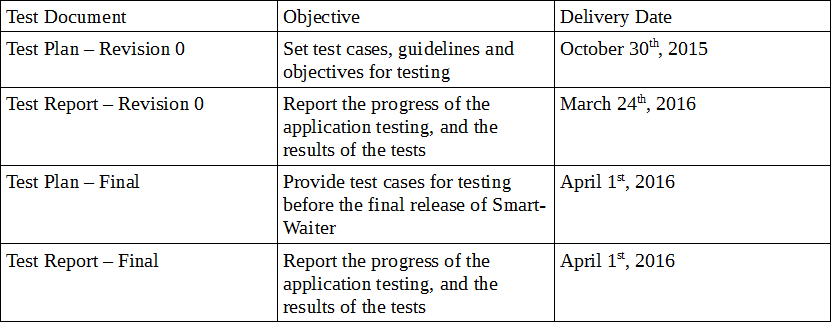
\includegraphics[width=\textwidth,height=\textheight,keepaspectratio]{TestingSchedule.png}


\end{document}
